\documentclass[11pt, compress, aspectratio=1610]{beamer}

\usetheme{pl}

% Set language
\usepackage{xstring}
\newcommand{\Langue}[1]{%
    \IfEqCase{#1}{%
        {francais}{
        \usepackage[utf8]{inputenc}
        \usepackage[francais]{babel}
        }%
        {english}{\usepackage[english]{babel}}%
    }[\PackageError{Langue}{Undefined option to language: #1}{}]%
}%
\Langue{francais}

% tikz diagrams
\usepackage{tikz}
\usetikzlibrary{shapes,snakes}
\usetikzlibrary{er}
\usetikzlibrary{arrows, plotmarks, decorations.markings}
\tikzstyle{arrow} = [->,>=stealth,thick,rounded corners=10pt,line width=0.1pt]
\usetikzlibrary{shadows}
\usetikzlibrary{shadings}
\usetikzlibrary{tikzmark, positioning, calc} % calc, to calculate coordinate
\tikzstyle{State}=[circle,
		thick,
		minimum size = 0.8cm,
		inner sep =5pt,
		draw=plST,
		fill=plST]

\usepackage{verbatim}
\usepackage{longtable}
\usepackage{booktabs}
\usepackage{minted}
\usepackage{listings}
\usepackage{color}
\usepackage{fancyvrb}
\newcommand{\VerbBar}{|}
\newcommand{\VERB}{\Verb[commandchars=\\\{\}]}
\DefineVerbatimEnvironment{Highlighting}{Verbatim}{commandchars=\\\{\},fontsize=\small}
% Add ',fontsize=\small' for more characters per line
\usepackage[framemethod=tikz]{mdframed}
\definecolor{shadecolor}{HTML}{EEEEEE}
\mdfsetup{
  backgroundcolor=shadecolor,
  linecolor=shadecolor,
  innerleftmargin=5pt,
  innerrightmargin=5pt,
  leftmargin=-5pt,
  rightmargin=-5pt,
  roundcorner=3pt
}
\newenvironment{Shaded}{\begin{mdframed}}{\end{mdframed}}
\newcommand{\KeywordTok}[1]{\textcolor[rgb]{0.26,0.66,0.93}{\textbf{{#1}}}}
\newcommand{\DataTypeTok}[1]{\textcolor[rgb]{0.74,0.68,0.62}{\underline{{#1}}}}
\newcommand{\DecValTok}[1]{\textcolor[HTML]{558B2F}{{#1}}}
\newcommand{\BaseNTok}[1]{\textcolor[HTML]{558B2F}{{#1}}}
\newcommand{\FloatTok}[1]{\textcolor[HTML]{558B2F}{{#1}}}
\newcommand{\ConstantTok}[1]{\textcolor[rgb]{0.74,0.68,0.62}{{#1}}}
\newcommand{\CharTok}[1]{\textcolor[HTML]{7E57C2}{{#1}}}
\newcommand{\SpecialCharTok}[1]{\textcolor[HTML]{7E57C2}{{#1}}}
\newcommand{\StringTok}[1]{\textcolor[HTML]{7E57C2}{{#1}}}
\newcommand{\VerbatimStringTok}[1]{\textcolor[HTML]{7E57C2}{{#1}}}
\newcommand{\SpecialStringTok}[1]{\textcolor[HTML]{7E57C2}{{#1}}}
\newcommand{\ImportTok}[1]{\textcolor[rgb]{0.74,0.68,0.62}{{#1}}}
\newcommand{\CommentTok}[1]{\textcolor[HTML]{546E7A}{\textit{{#1}}}}
\newcommand{\DocumentationTok}[1]{\textcolor[HTML]{BCAAA4}{\textit{{#1}}}}
\newcommand{\AnnotationTok}[1]{\textcolor[HTML]{BCAAA4}{\textbf{\textit{{#1}}}}}
\newcommand{\CommentVarTok}[1]{\textcolor[rgb]{0.74,0.68,0.62}{{#1}}}
\newcommand{\OtherTok}[1]{\textcolor[rgb]{0.74,0.68,0.62}{{#1}}}
\newcommand{\FunctionTok}[1]{\textcolor[HTML]{26A69A}{\textbf{{#1}}}}
\newcommand{\VariableTok}[1]{\textcolor[rgb]{0.74,0.68,0.62}{{#1}}}
\newcommand{\ControlFlowTok}[1]{\textcolor[rgb]{0.26,0.66,0.93}{\textbf{{#1}}}}
\newcommand{\OperatorTok}[1]{\textcolor[rgb]{0.74,0.68,0.62}{{#1}}}
\newcommand{\BuiltInTok}[1]{\textcolor[HTML]{42A5F5}{{#1}}}
\newcommand{\ExtensionTok}[1]{\textcolor[rgb]{0.74,0.68,0.62}{{#1}}}
\newcommand{\PreprocessorTok}[1]{\textcolor[rgb]{0.74,0.68,0.62}{\textbf{{#1}}}}
\newcommand{\AttributeTok}[1]{\textcolor[rgb]{0.74,0.68,0.62}{{#1}}}
\newcommand{\RegionMarkerTok}[1]{\textcolor[rgb]{0.74,0.68,0.62}{{#1}}}
\newcommand{\InformationTok}[1]{\textcolor[rgb]{0.00,0.40,1.00}{\textbf{\textit{{#1}}}}}
\newcommand{\WarningTok}[1]{\textcolor[HTML]{FF6E40}{\textbf{{#1}}}}
\newcommand{\AlertTok}[1]{\textcolor[HTML]{FF3D00}{{#1}}}
\newcommand{\ErrorTok}[1]{\textcolor[HTML]{DD2C00}{\textbf{{#1}}}}
\newcommand{\NormalTok}[1]{\textcolor[HTML]{212121}{{#1}}}
\newcommand\smallcitation[1]{% command to add small citation in the corner
\begin{textblock*}{\textwidth}(30pt,\textheight)
	\raggedleft \footnotesize\textit{#1}
\end{textblock*}}
\providecommand{\tightlist}{%
  \setlength{\itemsep}{0pt}\setlength{\parskip}{0pt}}

\let\OldTexttt\texttt
\renewcommand{\texttt}[1]{\OldTexttt{\color{plTT}#1}}

\makeatletter
\def\maxwidth{\ifdim\Gin@nat@width>\linewidth\linewidth\else\Gin@nat@width\fi}
\makeatother

\usepgfplotslibrary{dateplot}

\newcommand{\begincols}{\begin{columns}}
\newcommand{\stopcols}{\end{columns}}
\newcommand{\roundpicture}[2]{%
\tikz\node[circle,
          text=white,
          minimum width=4cm,
          minimum height=4cm,
          path picture={
              \node at (path picture bounding box.center){
                  \includegraphics[width=5cm]{#1}
              };
          }]{#2};
}
\newcommand{\plain}[1]{%
\begin{picture}(0,0)
  \put(-28.5,-175){%
      \pgfuseimage{titlebackground}
  }
  \put(0,-145){%
      \begin{minipage}[b][4.5cm][t]{0.5\textwidth}
          \color{plST}\huge
              #1
      \end{minipage}
  }
\end{picture}
}

\title{Lier l’aménagement forestier et \newline l’écologie théorique}
\subtitle{Adaptations aux changements climatiques}
\date{\today}
\author{Willian Vieira \& Dominique Gravel \newline}
\institute{}

\begin{document}

\maketitle

\begin{frame}{contexte}
\protect\hypertarget{contexte}{}

\centering{\large{Distribution d'aire de répartition}}

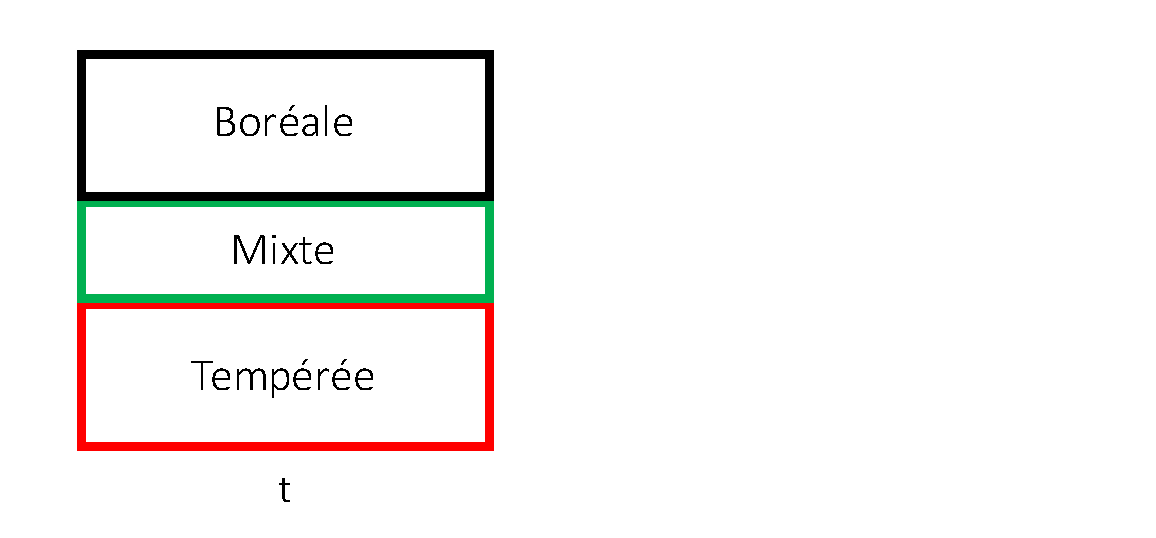
\includegraphics[scale=0.65]{figures/migration0.pdf}

\end{frame}

\begin{frame}{contexte}
\protect\hypertarget{contexte-1}{}

\centering{\large{Changement climatique}}

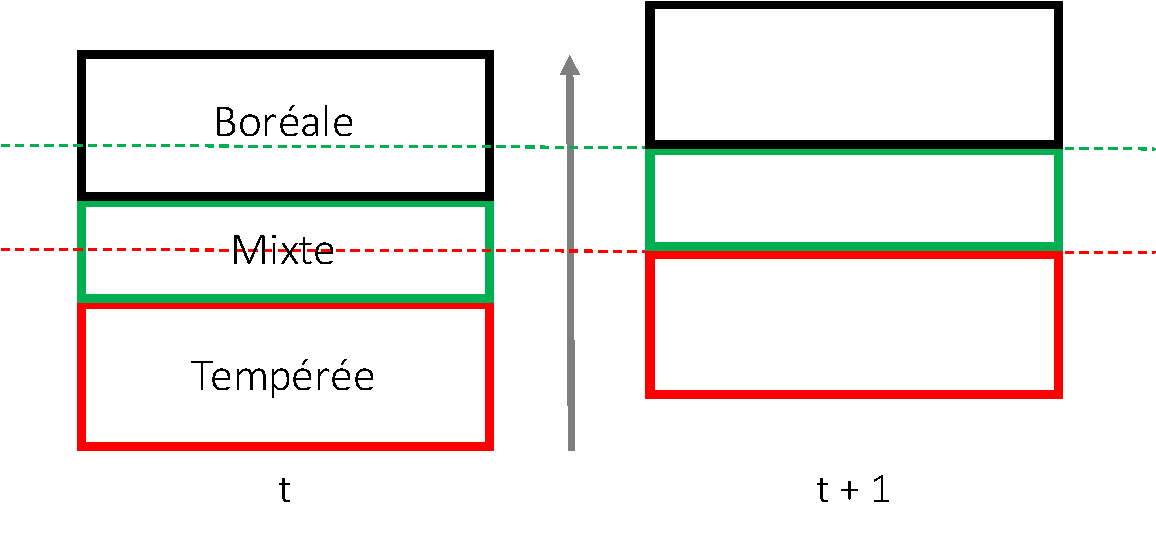
\includegraphics[scale=0.65]{figures/migration.pdf}

\end{frame}

\begin{frame}{contexte}
\protect\hypertarget{contexte-2}{}

\centering{\large{retard par rapport à la niche climatique}}

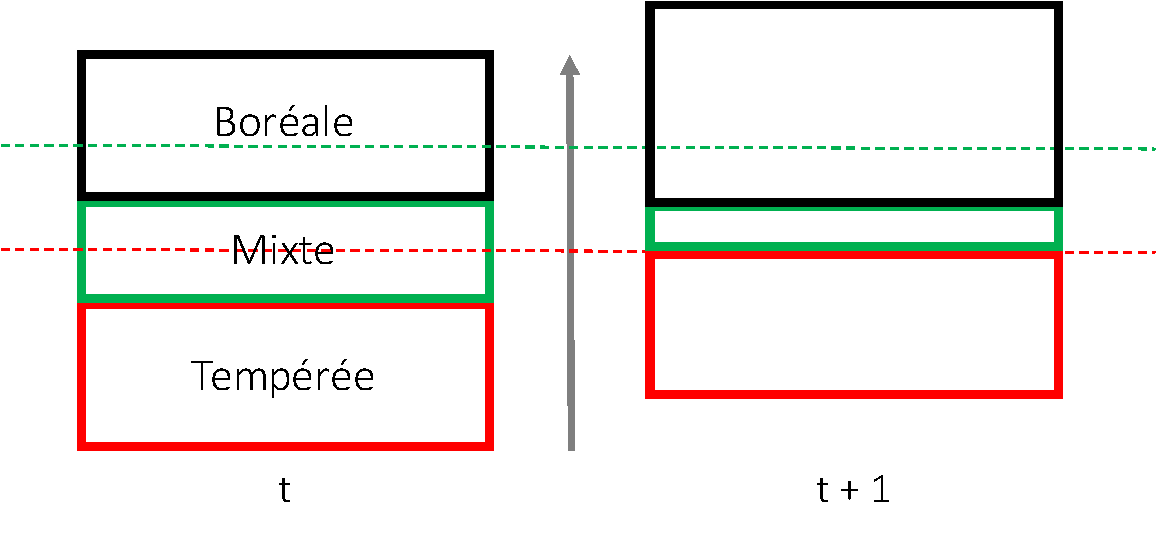
\includegraphics[scale=0.65]{figures/migration1.pdf}

\end{frame}

\begin{frame}{contexte}
\protect\hypertarget{contexte-3}{}

\centering{\large{rattraper avec l'aménagement forestier}}

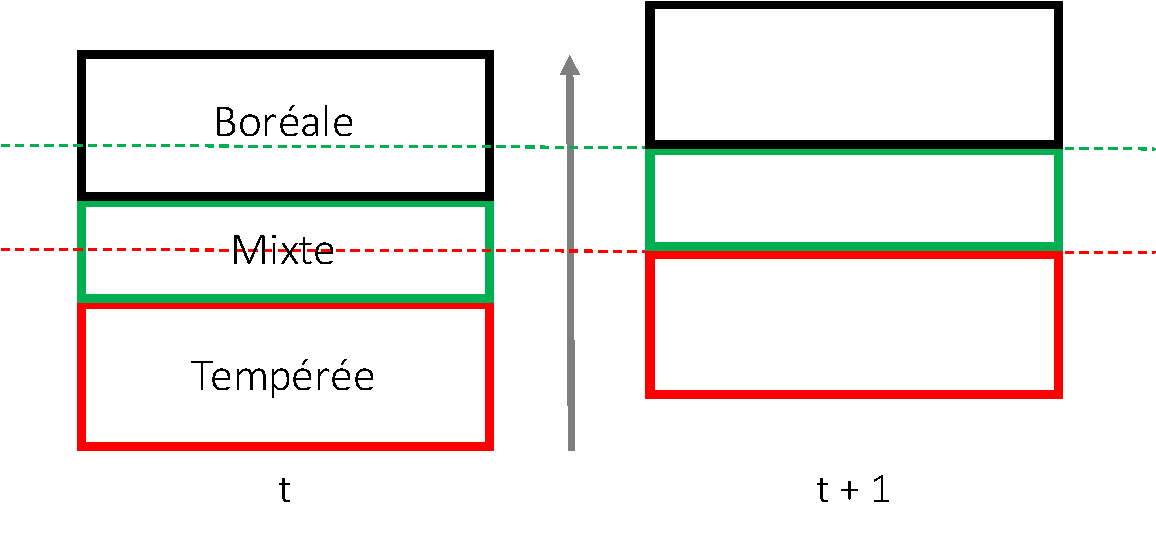
\includegraphics[scale=0.65]{figures/migration.pdf}

\end{frame}

\begin{frame}{Modèle}
\protect\hypertarget{moduxe8le}{}

\begincols
\column{0.48\textwidth}
  	\begin{tikzpicture}[->,>=stealth',auto,scale=0.45]
		\node [circle,StateM] (M) at (0,0) {\textcolor{white}{M}};
		\node [circle,StateB] (B) at (-8,5) {\textcolor{white}{B}};
		\node [circle,StateT] (T) at (8,5) {\textcolor{white}{T}};
		\node [circle,StateR] (R) at (0,10) {\textcolor{white}{R}};

		\path	(M) edge [thick,loop below,-latex]  node {} (M);
		\path	(T) edge [thick,loop right,-latex]  node {} (T);
		\path	(B) edge [thick,loop left,-latex]  node {} (B);
		\path	(R) edge [thick,loop above,-latex]  node {} (R);

		\draw[thick,-latex] (M) to node[above,sloped] {} (B);
		\draw[thick,-latex] (B) to[bend right=25] node[below,sloped] {} (M);

		\draw[thick,-latex] (T) to[bend left=25] node[below,sloped] {Colonisation} (M);
		\draw[thick,-latex] (M) to node[above,sloped] {Exclusion compétitive} (T);

		\draw[thick,-latex] (R) to[bend left=25] node[above,sloped] {Succession} (T);
		\draw[thick,-latex] (T) to node[below,sloped] {Pertubation} (R);

		\draw[thick,-latex] (R) to[bend right=25] node[above,sloped] {} (B);
		\draw[thick,-latex] (B) to node[below,sloped] {} (R);

		\draw[thick,-latex,transform canvas={xshift=0.8ex}] (R) to node[above,sloped] {} (M);
		\draw[thick,-latex,transform canvas={xshift=-0.8ex}] (M) to node[above,sloped] {} (R);
	\end{tikzpicture}

\hfill\column{0.35\textwidth}

\begin{description}
\tightlist
\item[B]
Boréale
\item[M]
Mixte
\item[T]
Tempérée
\item[R]
Régeneration
\end{description}

\stopcols

\end{frame}

\begin{frame}{Intégration avec l’aménagement forestier}
\protect\hypertarget{intuxe9gration-avec-lamuxe9nagement-forestier}{}

\centering

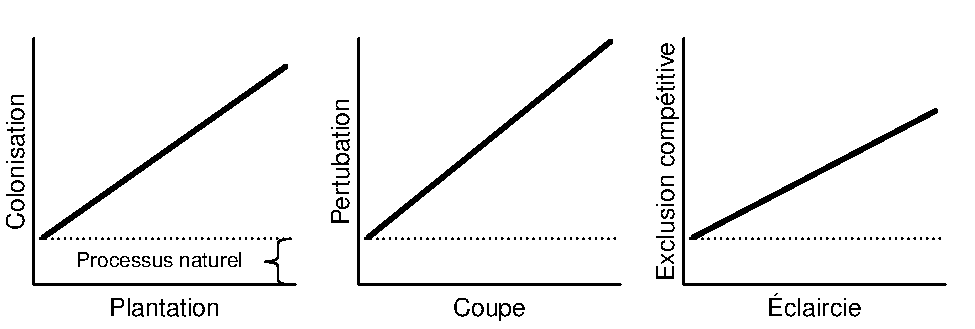
\includegraphics[scale=0.65]{figures/managMechanism.pdf}

\par

\end{frame}

\begin{frame}{Résultats préliminaires}
\protect\hypertarget{ruxe9sultats-pruxe9liminaires}{}

Effet de la \textbf{plantation} et de la \textbf{coupe}

\centering

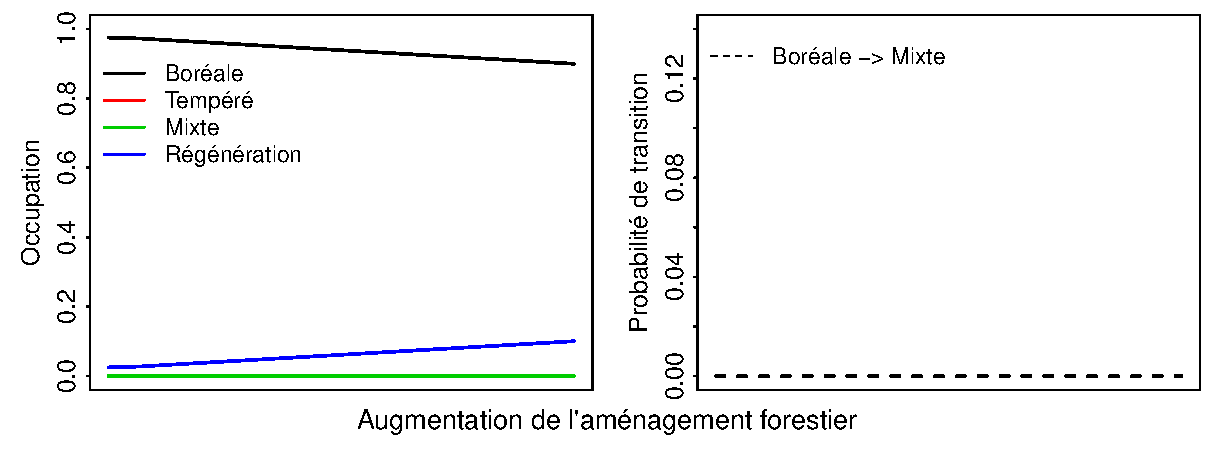
\includegraphics[scale=0.65]{figures/result0.pdf}

\par

\end{frame}

\begin{frame}{Résultats préliminaires}
\protect\hypertarget{ruxe9sultats-pruxe9liminaires-1}{}

Effet de l’\textbf{éclaircie}

\centering

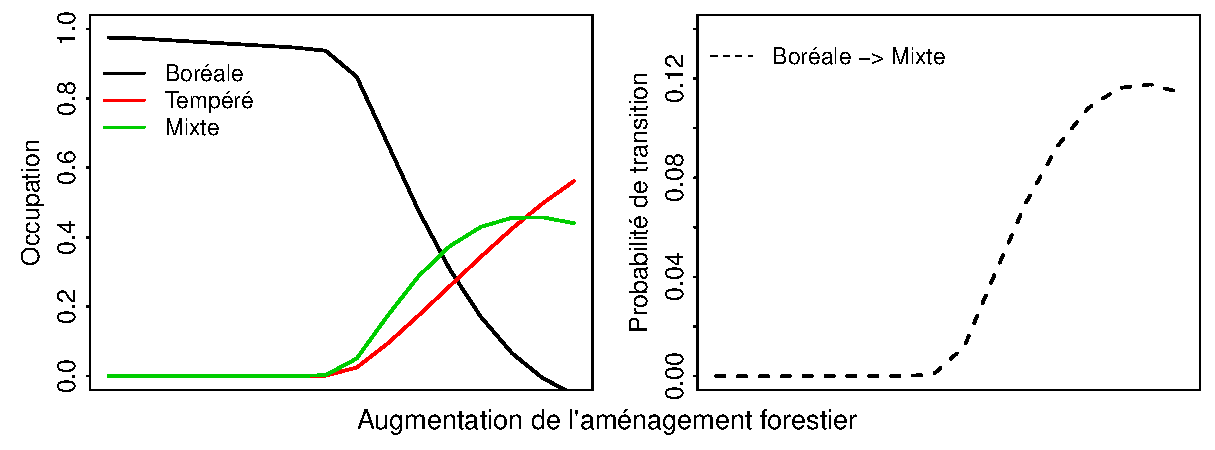
\includegraphics[scale=0.65]{figures/result1.pdf}

\par

\end{frame}

\begin{frame}{Importance des processus à l’échelle locale}
\protect\hypertarget{importance-des-processus-uxe0-luxe9chelle-locale}{}

\centering

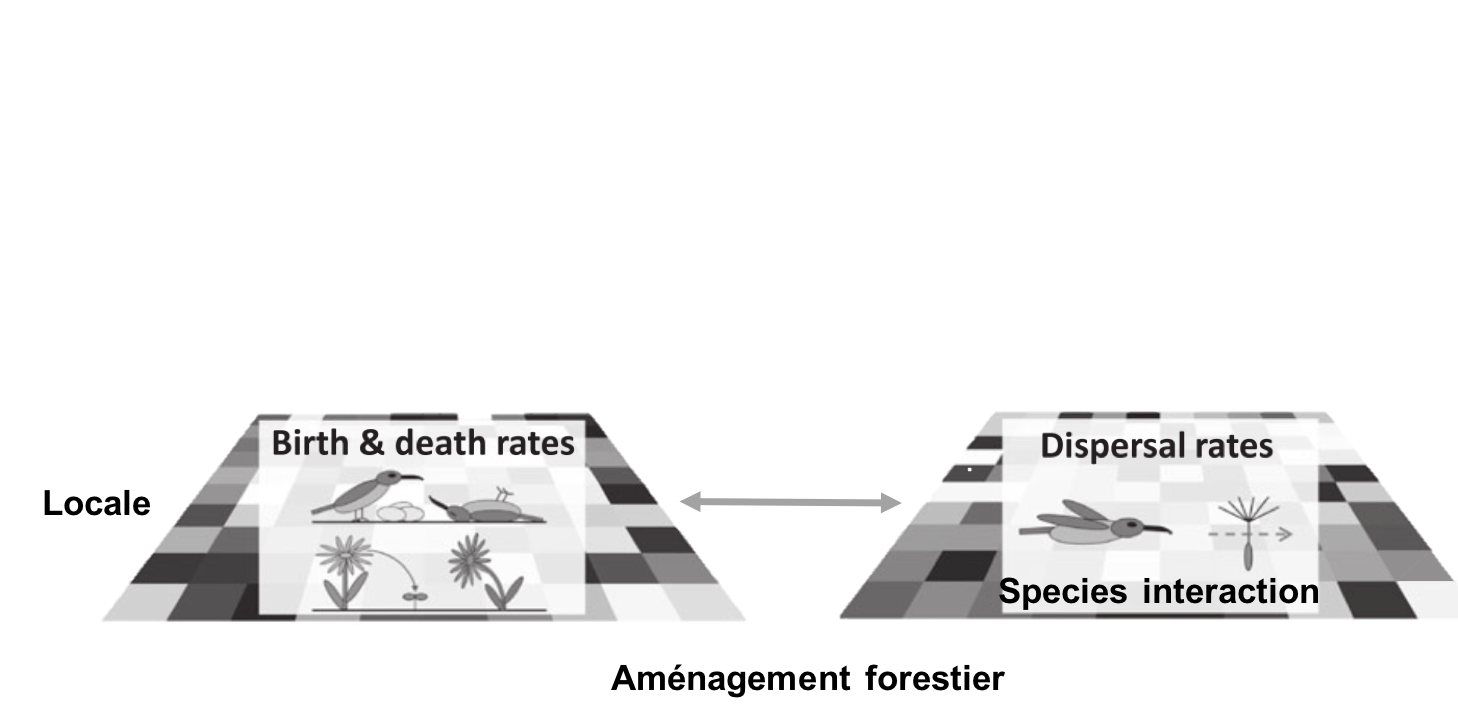
\includegraphics[scale=0.47]{figures/scaleInt.png}

\par

\smallcitation{Schurr \textit{et al}. 2012 \textit{J. Biogeogr.}}

\end{frame}

\begin{frame}{Importance des interactions entre échelles spatiales}
\protect\hypertarget{importance-des-interactions-entre-uxe9chelles-spatiales}{}

\centering

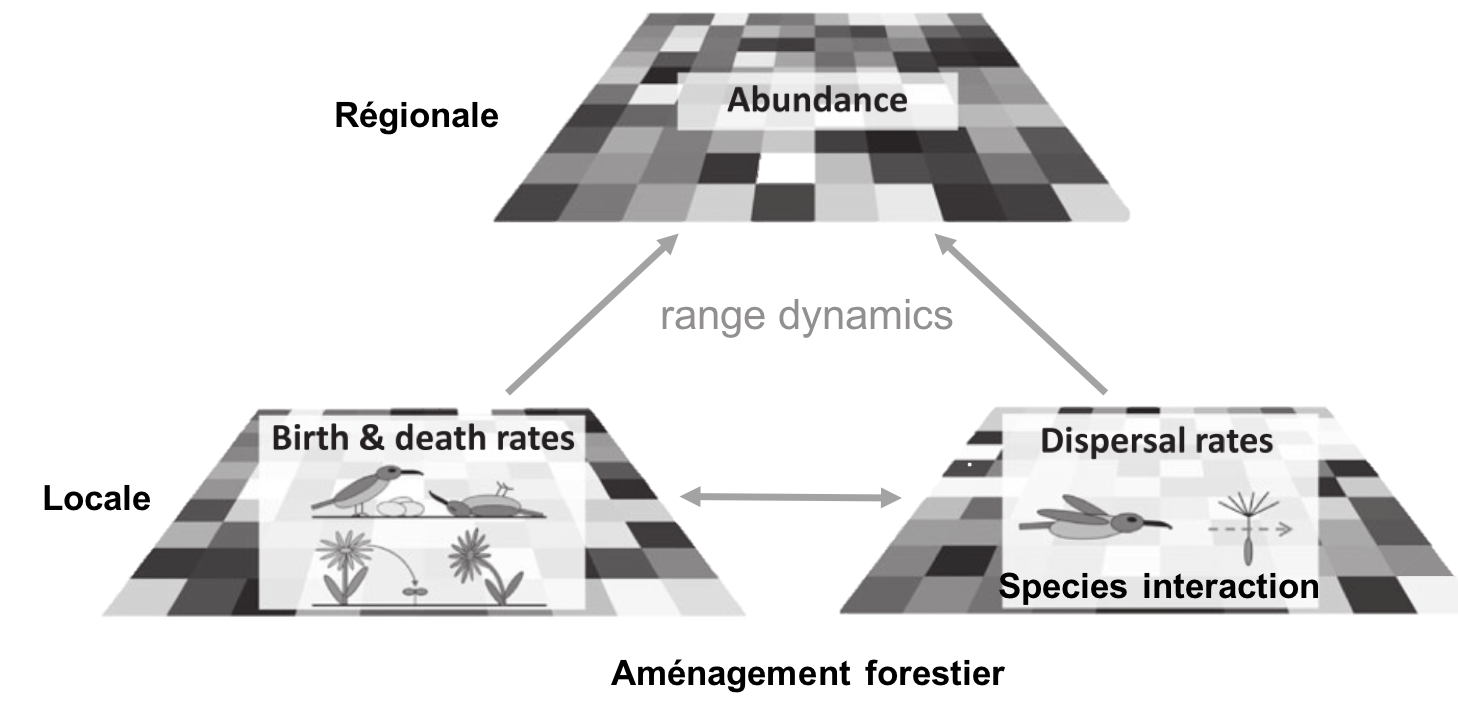
\includegraphics[scale=0.47]{figures/scaleInt1.png}

\par

\smallcitation{Schurr \textit{et al}. 2012 \textit{J. Biogeogr.}}

\end{frame}

\begin{frame}[plain]{}
\protect\hypertarget{section}{}

\plain{Thank you! \newline Merci !}

\end{frame}

\begin{frame}[plain]
  \begin{picture}(0,0)
    \put(-28.5,-175){%
      \pgfuseimage{titlebackground}
    }
  \end{picture}
\end{frame}

\end{document}
